\documentclass{article}
\usepackage[utf8]{inputenc}
\usepackage{graphicx}
\graphicspath{ {./images/} }
\usepackage{listings}

\title{CS 590 Assignment 5}
\author{Luke Jiang (jiang700@purdue.edu) }
\date{April 6, 2021}

\begin{document}

\maketitle

\section{Custom Service}
I modified and extended the \textit{time-service} given by the sample to include a greeting message based on the hour of the current hour. The modified code is the following:
\begin{verbatim}
    package main
    
    import (
        "net/http"
        "time"
        "github.com/gin-gonic/gin"
    )
    
    func main() {
        router := gin.Default()
    
        router.GET("/currenttime", currentTime)
    
        router.Run(":8082")
    }
    
    func currentTime(c *gin.Context) {
        currentTime := time.Now()
        hours, _, _ := currentTime.Clock()
        msg := ""
        if (hours < 6) {
          msg += "It's late night"
        } else if (hours < 10) {
          msg += "Good morning"
        } else if (hours < 13) {
          msg += "Good day"
        } else if (hours < 16) {
          msg += "Good afternoon"
        } else if (hours < 20) {
          msg += "Good evening"
        } else {
          msg += "Good night"
        }
    
        c.JSON(http.StatusOK, gin.H{
                "time": currentTime.Format("2006-01-02 3:4:5 pm"),
                "msg": msg,
        },
        )
    }
\end{verbatim}
I used the same Dockerfile to build the application, and used this config.json to create the pod:
\begin{verbatim}
    {
        "kind": "Pod",
        "apiVersion": "v1",
        "metadata": {
                "name": "time-application",
                "labels": {
                        "app": "webapp"
                }
        },
        "spec": {
                "containers": [
                        {
                                "name": "time-service",
                                "image": "time-service:latest",
                                "imagePullPolicy": "IfNotPresent",
                                "ports": [
                                        {
                                                "containerPort": 8082
                                        }
                                ],
                                "command": ["./main"]
                        }
                ]
        }
}
\end{verbatim}
Note that the \textit{containerPort} is specified as 8082. After the pod is created, I check the IP address of the pod:\\
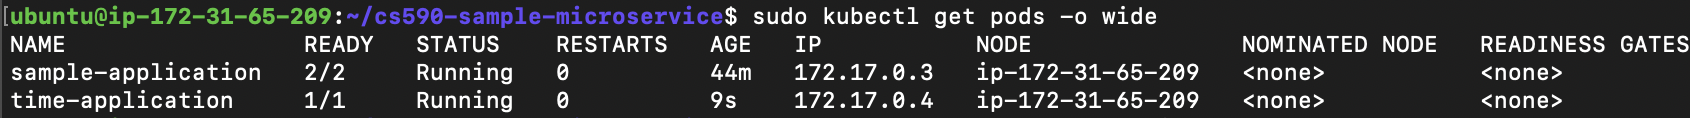
\includegraphics[scale=0.5]{ass5-ip.png}
And verified that my application is working:\\

\includegraphics[scale=0.5]{ass5-response.png}

\end{document}